\documentclass[a5paper, 12dd, twoside]{article}
% !TeX spellcheck = ru_RU
%Автор - Краснов Александр 2022

%Настройка языка и отображения
\usepackage[russian]{babel}
%Шрифты
\usepackage[T2A]{fontenc}		%Русские шрифты
%\usefont{T2A}{Tempora-TLF}{m}{n}
%\usepackage{lmodern}			%Шрифт Latin Modern, нужен если нет cm-super

\usepackage[utf8]{inputenc}		%Кодировка
\usepackage{amssymb,amsmath}	%Математические символы
\usepackage{multicol}			%Несколько колонок
%\usepackage{color}				%Использовать цветной текст

\usepackage{graphicx}			%Пикчи
\DeclareGraphicsExtensions{.pdf,.png,.jpg}
\frenchspacing					%Отключает большой пробел между предложениями

\usepackage{indentfirst}		%Красная строка
\setlength{\parindent}{1.25cm}	%Настройка отступа красной строки для шрифта 14pt, по умолчанию 15pt
\linespread{1.25} 				%Межстрочный интервал

\usepackage{parskip} 			%Интервал между абзацами
\setlength{\parindent}{1cm} 	%Настройка интервала между абзацами, по умолчанию будет 0

\usepackage{enumitem}			%Настройка списков
\setlist{noitemsep}				%Убирает лишнюю строку в списках

\usepackage{textcomp}			%Улучшает знак номера

\usepackage{cmap}				%Ссылки в PDF
\usepackage[					%Гипертекстовое оглавление в PDF
bookmarks=true, colorlinks=true, unicode=true,
urlcolor=black,linkcolor=black, anchorcolor=black,
citecolor=black, menucolor=black, filecolor=black,
]{hyperref}

%\sloppy						%Автоматическое разряжение строк (только для черновиков)
\emergencystretch=20pt			%Аварийное разряжение строк (подбор опытным путем)
%\hfuzz=0.5pt					%Разрешить переполнение абзаца на 0.5dd (выглядит приемлемо)
\tolerance=300					%Настройка максимальной разряженности строки
\hyphenpenalty=100				%Настройка частоты переносов

\clubpenalty=5000				%Настройка висячих строк в начале абзаца от 0 до 10000
\widowpenalty=5000				%настройка висячих строк в конце абзаца от 0 до 10000


%Колонтитулы и номера страниц
%\pagestyle{empty} 				%Нет ни колонтитулов, ни номеров страниц
\pagestyle{plain} 				%Номера страниц ставятся внизу в середине строки, колонтитулов нет
%\pagestyle{headings} 			%Присутствуют колонтитулы (включающие в себя и номера страниц)
%\pagestyle{myheadings}			%То же, что и headings, но делается вручную

\pagenumbering{arabic}			%Нумерация страниц арабскими цифрами
%\pagenumbering{roman}			%Нумерация страниц римскими строчными цифрами
%\pagenumbering{Roman}			%Нумерация страниц римскими заглавными цифрами
%\pagenumbering{alph}			%Нумерация страниц строчными английскими буквами
%\pagenumbering{Alph}			%Нумерация страниц заглавными английскими буквами
%\pagenumbering{asbuk}			%Нумерация страниц строчными русскими буквами
%\pagenumbering{Asbuk}			%Нумерация страниц заглавными русскими буквами


%\usepackage{fancyhdr}			%Колонтитулы
%\pagestyle{fancy} 				%Использование кастомных колонтитулов
%\fancyhf{} 					%Отчистить все колонтитулы
%\lhead{} 						% левый верхний колонтитул
%\chead{} 						% центральный верхний
%\rhead{} 						% правый верхний
%\lfoot{} 						% левый нижний
%\cfoot{\thepage} 				% центральный нижний
%\rfoot{} 						% правый нижний


\usepackage{listings}
% настройка подсветки кода и окружения для листингов
%\usemintedstyle{colorful}
%\newenvironment{code}{\captionsetup{type=listing}}{}


%Спецсимволы
\usepackage{wasysym}			%Специальные символы, в том числе и гачи
\newcommand{\gachi}{\male}		%Гачи значок


%реализовать модификаторы шрифтов горячими клавишами



%Настройки верстки
%\openany						%Глава может начинаться с любой страницы
%\openright						%Глава только с правой страницы

%\fleqn							%Формулы слева
%\leqno							%Номера формул слева

%\raggedbottom					%Страницы разной высоты
\flushbottom					%Страницы одинаковой высоты

%\columnseprule=0.4pt			%Ширина линейки при верстке в колонки
%\columnsep=0mm					%Расстояние между колонками при верстке в колонки


%Настройка страниц

\usepackage[left=1.5cm, right=1.5cm, top=1.5cm, bottom=1.5cm]{geometry}
%twoside, openany,%
\hyphenation{
    про-из-вод-стве 
    до-пус-ти-мых 
    тех-но-ло-ги-чес-ких 
    рес-пи-ра-то-ров 
    про-вес-ти 
    э-лек-тро-маг-нит-но-го 
    ста-ти-сти-чес-ким 
    са-мо-сто-я-тель-но 
    ко-леб-лю-ще-го-ся 
    им-пульс-но-го 
    ус-та-нав-ли-ва-ют 
    не-пос-то-ян-но-го 
    ха-рак-те-рис-ти-ки
    про-из-вод-ствен-но-го 
    про-ме-жу-ток 
    пос-ле-ду-ю-щей
    раз-ве-ва-ю-щи-е-ся
    сви-са-ю-щи-е
    пред-ме-ты
    ре-зуль-та-те
    о-бес-то-чен
    за-кре-пи-те
    вни-ма-тель-ны
    и-зо-ля-ци-ю
    ком-плек-ту-ю-щи-е
    поз-во-ля-ет
    прак-ти-чес-ки
    об-ду-мать
    по-верх-нос-ти
    по-ло-же-ний
    по-лез-ность
    сто-ро-ной
    кон-струк-тив-но-го
    о-со-бен-нос-ти
    по-ни-ма-ния
    не-об-хо-ди-мые
    зна-ко-мых
    ис-поль-зу-ют-ся
    у-вле-ка-тель-ная
    ро-бо-то-тех-ни-ки
    у-прав-лять
    ин-струк-ци-ям
    у-да-лен-но
    функ-ци-о-наль-ность
    мо-ду-лю
    це-лом
    спе-ци-аль-нос-ти
    про-цесс
    об-щие
    по-лу-чи-ли
    ра-бо-та-ли
    тех-но-ло-ги-чес-кий
    ба-лан-си-ров-ки
    по-мощью
    ре-гу-ли-ру-ет-ся
    ско-рость
    от-но-си-тель-ную
    оп-ре-де-лять
    ком-пью-тер
    сиг-на-лы
    э-та-лон-ным
    пред-став-лен-но-го
    об-ра-зом
    пред-пи-сан-но-го
    пре-пят-ствий
    до-пол-ни-тель-ный
    преи-му-щест-ва
    кон-струк-ции
    за-клю-ча-ет-ся
    за-тра-ты
    на-мно-го
    сис-те-мах
    кон-ту-ру
    пе-ре-ход-ной
    ос-но-ве
    рас-сто-я-ние
    ос-лаб-ле-ние
    бла-го-да-ря
    за-мкну-то-му
    вы-со-кие
    ус-та-нов-ле-ния
    от-сле-жи-вать
    дат-чи-ка
    пред-став-лен-ный
    вклю-ча-ют
    по-мех
    от-ка-зов
    ис-поль-зо-ва-ние
    не-до-стат-ки
    на-прав-ле-ние
    от-ра-жа-тель-ной
    по-ло-же-ние
    раз-вер-нут
    сан-ти-мет-ры
    де-мон-стри-рует
    ин-же-нер-ных
    рас-счи-тан
    ба-лан-си-ру-ет
    сер-во-при-вод
    про-пор-ционал
    ал-го-ри-тм
    ко-то-рое
    по-ло-же-ния
    те-че-ни-ем
    по-лу-ча-ет
    сис-те-ма
    каж-дым
    уси-ле-ния
    ко-эф-фи-ци-ен-ты
    поль-зо-ва-те-лем
    ди-апа-зо-на
    от-но-си-тель-но
    зна-че-ния
    за-дан-но-го
    со-ед-и-не-нию
    дат-чи-ки
    вра-ще-ния
    из-ме-ря-ет
    ме-ха-ни-зма-ми
    ко-то-рый
    не-гра-ви-та-ци-он-ное
    прог-рам-ми-ро-ва-ние
    про-ф-ес-си-о-на-ль-ной
    де-я-т-е-ль-но-с-ти
    фор-ми-ро-ва-ние
    про-фес-сио-наль-ное
    ин-фор-ма-ции
    дея-тель-нос-ти
    до-к-у-м-ен-та-ц-ии
    при-ме-ни-тель-но
    об-о-р-у-до-ва-н-ия
    со-ци-аль-но-го
    не-об-хо-ди-мо-го
    го-су-дар-ст-вен-ном
    ис-поль-зо-вать
    сред-ст-ва
    фи-зи-чес-кой
    куль-ту-ры
    сох-ра-не-ния
    ук-р-е-п-л-е-н-ия
    про-цес-се
    под-дер-жа-ние
    не-об-хо-ди-мо-го
    фи-зи-чес-кой
    под-го-тов-лен-нос-ти
    вы-би-рать
    спо-со-бы
    ре-ше-ния
    про-фес-сио-наль-ной
    при-ме-ни-тель-но
    раз-лич-ным
    кон-тек-с-там
    мон-таж
    прог-рам-ми-ро-ва-ние
    ме-ха-трон-ных
    мо-биль-ных
    ро-бо-то-тех-ни-чес-ких
    ком-плек-сов
    осу-щ-еств-лять
    нас-т-рой-ку
    кон-фи-гу-ри-ро-ва-ние
    про-г-рам-ми-ру-е-мых
    ло-ги-чес-ких
    кон-т-рол-ле-ров
    мик-р-о-про-цес-со-р-ных
    си-с-тем
    со-от-ве-т-ст-вии
    при-н-ци-пи-аль-ны-ми
    сх-е-ма-ми
    под-к-лю-че-ния
    раз-р-а-б-а-т-ы-в-ать
    уп-ра-в-ля-ю-щие
    прог-рам-мы
    ме-ха-тр-он-ных
    си-с-т-ем
    мо-б-иль-ных
    тех-ни-че-с-ким
    ре-а-ли-за-ц-ии
    не-о-че-ви-д-н-ых
    ис-то-ч-ни-к-ов
    гл-а-в-н-ых
    па-ра-ме-т-ра-ми
    са-мо-об-ра-зо-ва-н-ия
    пр-о-г-рам-ми-ро-ва-н-ия
    ан-а-л-о-го-в-ых
    раз-ра-бо-т-ке
    ра-бо-ты
    со-ци-аль-н-ом
    см-еж-н-ых
    ха-ра-к-те-р-н-ы-ми
    пр-оф-е-с-си-о-на-ль-н-ых
    из-в-е-ст-н-ые
    пла-ни-ру-е-м-ые
    ме-х-а-т-ро-н-н-ыми
    пр-и-хо-дит-ся
    об-л-ас-т-ях
    пр-о-ф-ес-с-и-о-на-ль-н-ые
    пр-о-ф-ес-с-и-о-на-ль-н-ая
    пр-о-из-но-ше-н-ия
    ра-б-о-ч-е-го
    вн-ут-рен-ней
    ка-че-ст-ве
    уп-ра-в-ле-ния
    дви-же-ния
    кн-о-п-ку
    си-с-т-е-ме
    до-ку-мен-та-ции
    про-фес-сии
    про-фес-си-о-наль-ному
    вы-п-о-л-н-е-н-ии
    по-ляр-но-сть
    про-г-р-а-м-ме
    по-ме-няй-те
    ре-в-е-рс
    ком-пь-ю-те-ру
    уп-рав-ля-ю-щая
    по-сле-до-ва-тель-но-с-ти
    про-ве-р-ок
    ком-би-на-ци-он-н-ых
    ре-з-уль-та-т-ом
    не-ис-п-ра-в-но-с-ть
    вк-лю-че-н-но-го
    не-ис-п-рав-но-с-ти
    ды-ма
    вн-е-ш-н-ий
    ло-ги-чес-к-ие
    сх-е-мы
    пр-и-ме-н-ен
    мо-ж-но
    об-ус-лов-ле-но
    ко-н-т-ро-ль-н-ую
    ми-к-ро-с-х-ем
    пр-е-д-с-та-в-ить
    со-от-вет-ст-во-ва-ть
    це-пи
    ос-цил-ло-гра-фи-ро-ва-ние
    кон-т-ро-ль-ных
    эл-ек-т-ри-чес-ких
    эл-ек-т-ро-о-бо-ру-до-ва-нии
    срав-ни-ва-ют
    ис-пы-та-ние
    вы-пол-не-нии
    TET-R-IX
    негр-а-ви-та-ци-он-ное
    объ-е-ди-ня-ют-ся
    ко-н-т-ро-л-лер
    ур-ав-но-ве-сить
    ком-п-л-ект
    по-в-ре-ж-де-н-ий
    эл-е-к-т-ри-ч-ес-к-им
    тра-в-мы
    из-л-о-жен-ны-ми
    пн-е-в-ма-ти-че-с-к-ой
    ма-ги-с-тра-ли
    из-бе-жа-н-ии
    со-е-д-и-не-н-ий
    ус-т-а-н-о-в-ки
    не-об-хо-ди-мос-ти
    об-с-лу-жи-в-а-н-ие
    на-деж-ность
    эл-е-к-т-ри-ч-ес-к-и-ми
    си-с-те-мы
    поль-з-у-й-тесь
    пред-наз-на-чен
    раз-лич-но-го
    уро-в-ень
    ри-с-у-нок
    ос-но-в-н-ой
    про-мыш-лен-ных
    объ-ек-та-ми
    ме-тал-ли-че-с-к-ий
    тем-пе-ра-ту-рах
    мес-т-ах
    соз-да-ния
    фор-ми-ру-е-т-ся
    уни-вер-са-ль-ным
    ав-то-ма-ти-за-ции
    энер-го-не-за-ви-си-мую
    язы-ке
    от-к-р-ы-тия
    вы-п-о-л-н-я-е-мых
    фи-з-и-че-с-кие
    об-р-а-бо-т-ки
    }

\title{Практическое занятие №1\\<<Выполнение расчета уровня шума на рабочем месте>>}
\author{Краснов Александр МР--19}


\begin{document}
\maketitle
\tableofcontents
\clearpage

\subsubsection*{Цель работы}
Овладение практическими навыками измерений шума с пос\-ле\-ду\-ю\-щей оценкой условий труда на рабочем месте.

\subsubsection*{Задачи}
Самостоятельно изучить основные физические ха\-рак\-те\-рис\-ти\-ки звука, классификацию производственного шума, его вредное действие на организм человека, нормирование; получить практические навыки измерений приборами уровней шума от различных источников; произвести расчеты эквивалентного уровня звука на рабочем месте; сравнить эффективность различных методов защиты от про\-из\-вод\-ствен\-но\-го шума.

\section{Шум}
{\itshape Шум} --- это звук, оцениваемый негативно и наносящий\- вред здоровью. 
В качестве звука человек воспринимает упругие колебания, распространяющиеся в среде, которая может быть твердой, жидкой или газообразной. В зависимости от источника генерирующего колебания, различают шумы механического, аэродинамического и электромагнитного происхождения. 

\subsection{Механический шум}
На ряде производств преобладает механический шум, основными источниками которого являются зубчатые передачи, механизмы ударного типа, цепные передачи, подшипники качения и т.п. Он вызывается силовыми воздействиями неуравновешенных вращающихся масс, ударами в сочленениях деталей, стуками в зазорах, движением материалов в трубопроводах и т.п. Спектр механического шума занимает широкую область частот. Определяющими факторами механического шума являются форма, размеры и тип конструкции, число оборотов, механические свойства материала, состояние поверхностей взаимодействующих тел и их смазывание. Машины ударного действия, к которым относится, например, кузнечно-прессовое оборудование, являются источником импульсного шума, причем его уровень на рабочих местах, как правило, превышает допустимый. На машиностроительных предприятиях наибольший уровень шума создается при работе метало -- и деревообрабатывающих станков. 

\subsection{Аэродинамические и гидродинамические шумы}
\begin{enumerate}
    \item шумы, обусловленные периодическим выбросом газа в ат\-мос\-фе\-ру, работой винтовых насосов и компрессоров, пневматических двигателей, двигателей внутреннего сгорания
    \item шумы, возникающие из-за образования вихрей потока у твердых границ. Эти шумы наиболее характерны для вентиляторов, турбовоздуходувок, насосов, турбокомпрессоров, воздуховодов
    \item кавитационный шум, возникающий в жидкостях из-за потери жидкостью прочности на разрыв при уменьшении давления ниже определенного предела и возникновения полостей и пузырьков, заполненных парами жидкости и растворенными в ней газами.
\end{enumerate}

\subsection{Шумы электромагнитного происхождения}
Шумы электромагнитного происхождения возникают в различных электротехнических изделиях (например, при работе электрических машин). Их причиной является взаимодействие ферримагнитных масс под влиянием переменных во времени и пространстве магнитных полей. Электрические машины создают шумы с различными уровнями звука от \(\frac{20}{30}\) дБ (микромашины) до \(\frac{20}{30}\) дБ (крупные быстроходные машины).

\section{Классификация шумов, воздействующих на человек}
\subsection{По характеру спектра шум делится}
\begin{enumerate}
    \item на широкополосный шум, с непрерывным спектром шириной более 1 октавы
    \item на тональный шум, в спектре которого имеются выраженные тоны
\end{enumerate}
Тональный характер шума для практических целей устанавливается измерением в \(\frac{1}{3}\) октавных полосах частот по превышению уровня в одной полосе над соседними не менее чем на 10 дБ.
\subsection{По временным характеристикам шум делится}
\begin{enumerate}
    \item на постоянный шум, уровень звука которого за 8-часовой рабочий день или за время измерения в помещениях жилых и общественных зданий, на территории жилой застройки изменяется во времени не более чем на 5 дБА
    \item непостоянный шум, уровень которого за 8-часовой рабочий день, рабочую смену или во время измерения в помещениях жилых и общественных зданий, на территории жилой застройки изменяется во времени более чем на 5 дБА
\end{enumerate}
\subsection{Непостоянные шумы подразделяют}
\begin{enumerate}
    \item на колеблющийся во времени шум, уровень звука которого непрерывно изменяется во времени
    \item прерывистый шум, уровень звука которого ступенчато изменяется на 5дБА и более, причем длительность интервалов, в течение которых уровень остается постоянным, составляет 1 с и более
    \item импульсный шум, состоящий из одного или нескольких звуковых сигналов, каждый длительностью менее 1 с, при этом уровни звука в дБАI и дБА отличаются не менее чем на 7 дБ.
\end{enumerate}

\section{Методы измерения шума на рабочих местах}
В соответствии с ГОСТ 12.1.050-86 «Методы измерения шума на рабочих местах»
\begin{enumerate}
    \item Микрофон следует располагать на высоте 1,5 м над уровнем пола или рабочей площадки (если работа выполняется стоя) или на высоте уха человека, подвергающегося воздействию шума (если работа выполняется сидя). Микрофон должен быть ориентирован в направлении максимального уровня шума и удален не менее чем на 0,5 м от оператора, проводящего измерения.
    \item Для оценки шума на постоянных рабочих местах измерения следует проводить в точках, соответствующих установленным постоянным местам.
    \item Для оценки шума на непостоянных рабочих местах измерения следует проводить в рабочей зоне в точке наиболее частого пребывания работающего.
    \item При проведении измерений октавных уровней звукового давления переключатель частотной характеристики прибора устанавливают в положение "фильтр". Октавные уровни звукового давления измеряют в полосах со среднегеометрическими частотами 63-8000 Гц. При проведении измерений уровней звука и эквивалентных уровней звука, дБА, переключатель частотной характеристики прибора устанавливают в положение ``А''.
    \item При проведении измерений уровней звука и октавных уровней звукового давления постоянного шума переключатель временной характеристики прибора устанавливают в положение ``медленно''. Значения уровней принимают по средним показателям при колебании стрелки прибора.
    \item Значения уровней звука и октавных уровней звукового давления считывают со шкалы прибора с точностью до 1 дБА, дБ.
    \item Измерения уровней звука и октавных уровней звукового давления постоянного шума должны быть проведены в каждой точке не менее трех раз.
    \item При проведении измерений эквивалентных уровней звука колеблющегося во времени шума для определения эквивалентного (по энергии) уровня звука переключатель временной характеристики прибора устанавливают в положение ``медленно''. Значения уровней звука принимают по показаниям стрелки прибора в момент отсчета.
    \item При проведении измерений максимальных уровней звука колеблющегося во времени шума переключатель временной характеристики прибора устанавливают в положение ``медленно''. Значения уровней звука снимают в момент максимального показания прибора.
    \item При проведении измерений максимальных уровней звука импульсного шума переключатель временной характеристики прибора устанавливают в положение ``импульс''. Значения уровней принимают по максимальному показанию прибора.
    \item Интервалы отсчета уровней звука колеблющегося во времени шума при измерениях эквивалентного уровня продолжительностью 30 мин составляют 5–6 с при общем числе отсчетов 360.
    \item При проведении измерений эквивалентных уровней звука непостоянного шума переключатель временной характеристики прибора устанавливают в положение ``медленно'', измеряют уровни звука и продолжительность каждой ступени.
\end{enumerate}

\section{Измерение шума на рабочем месте}
В ходе данной работы проводилось измерение уровня шума от системы охлаждения персонального компьютера (ноутбука) на рабочем месте. Микрофон располагался на уровне головы человека. Измерения проводились 3 раза.

\begin{figure}[p]
    \centering
    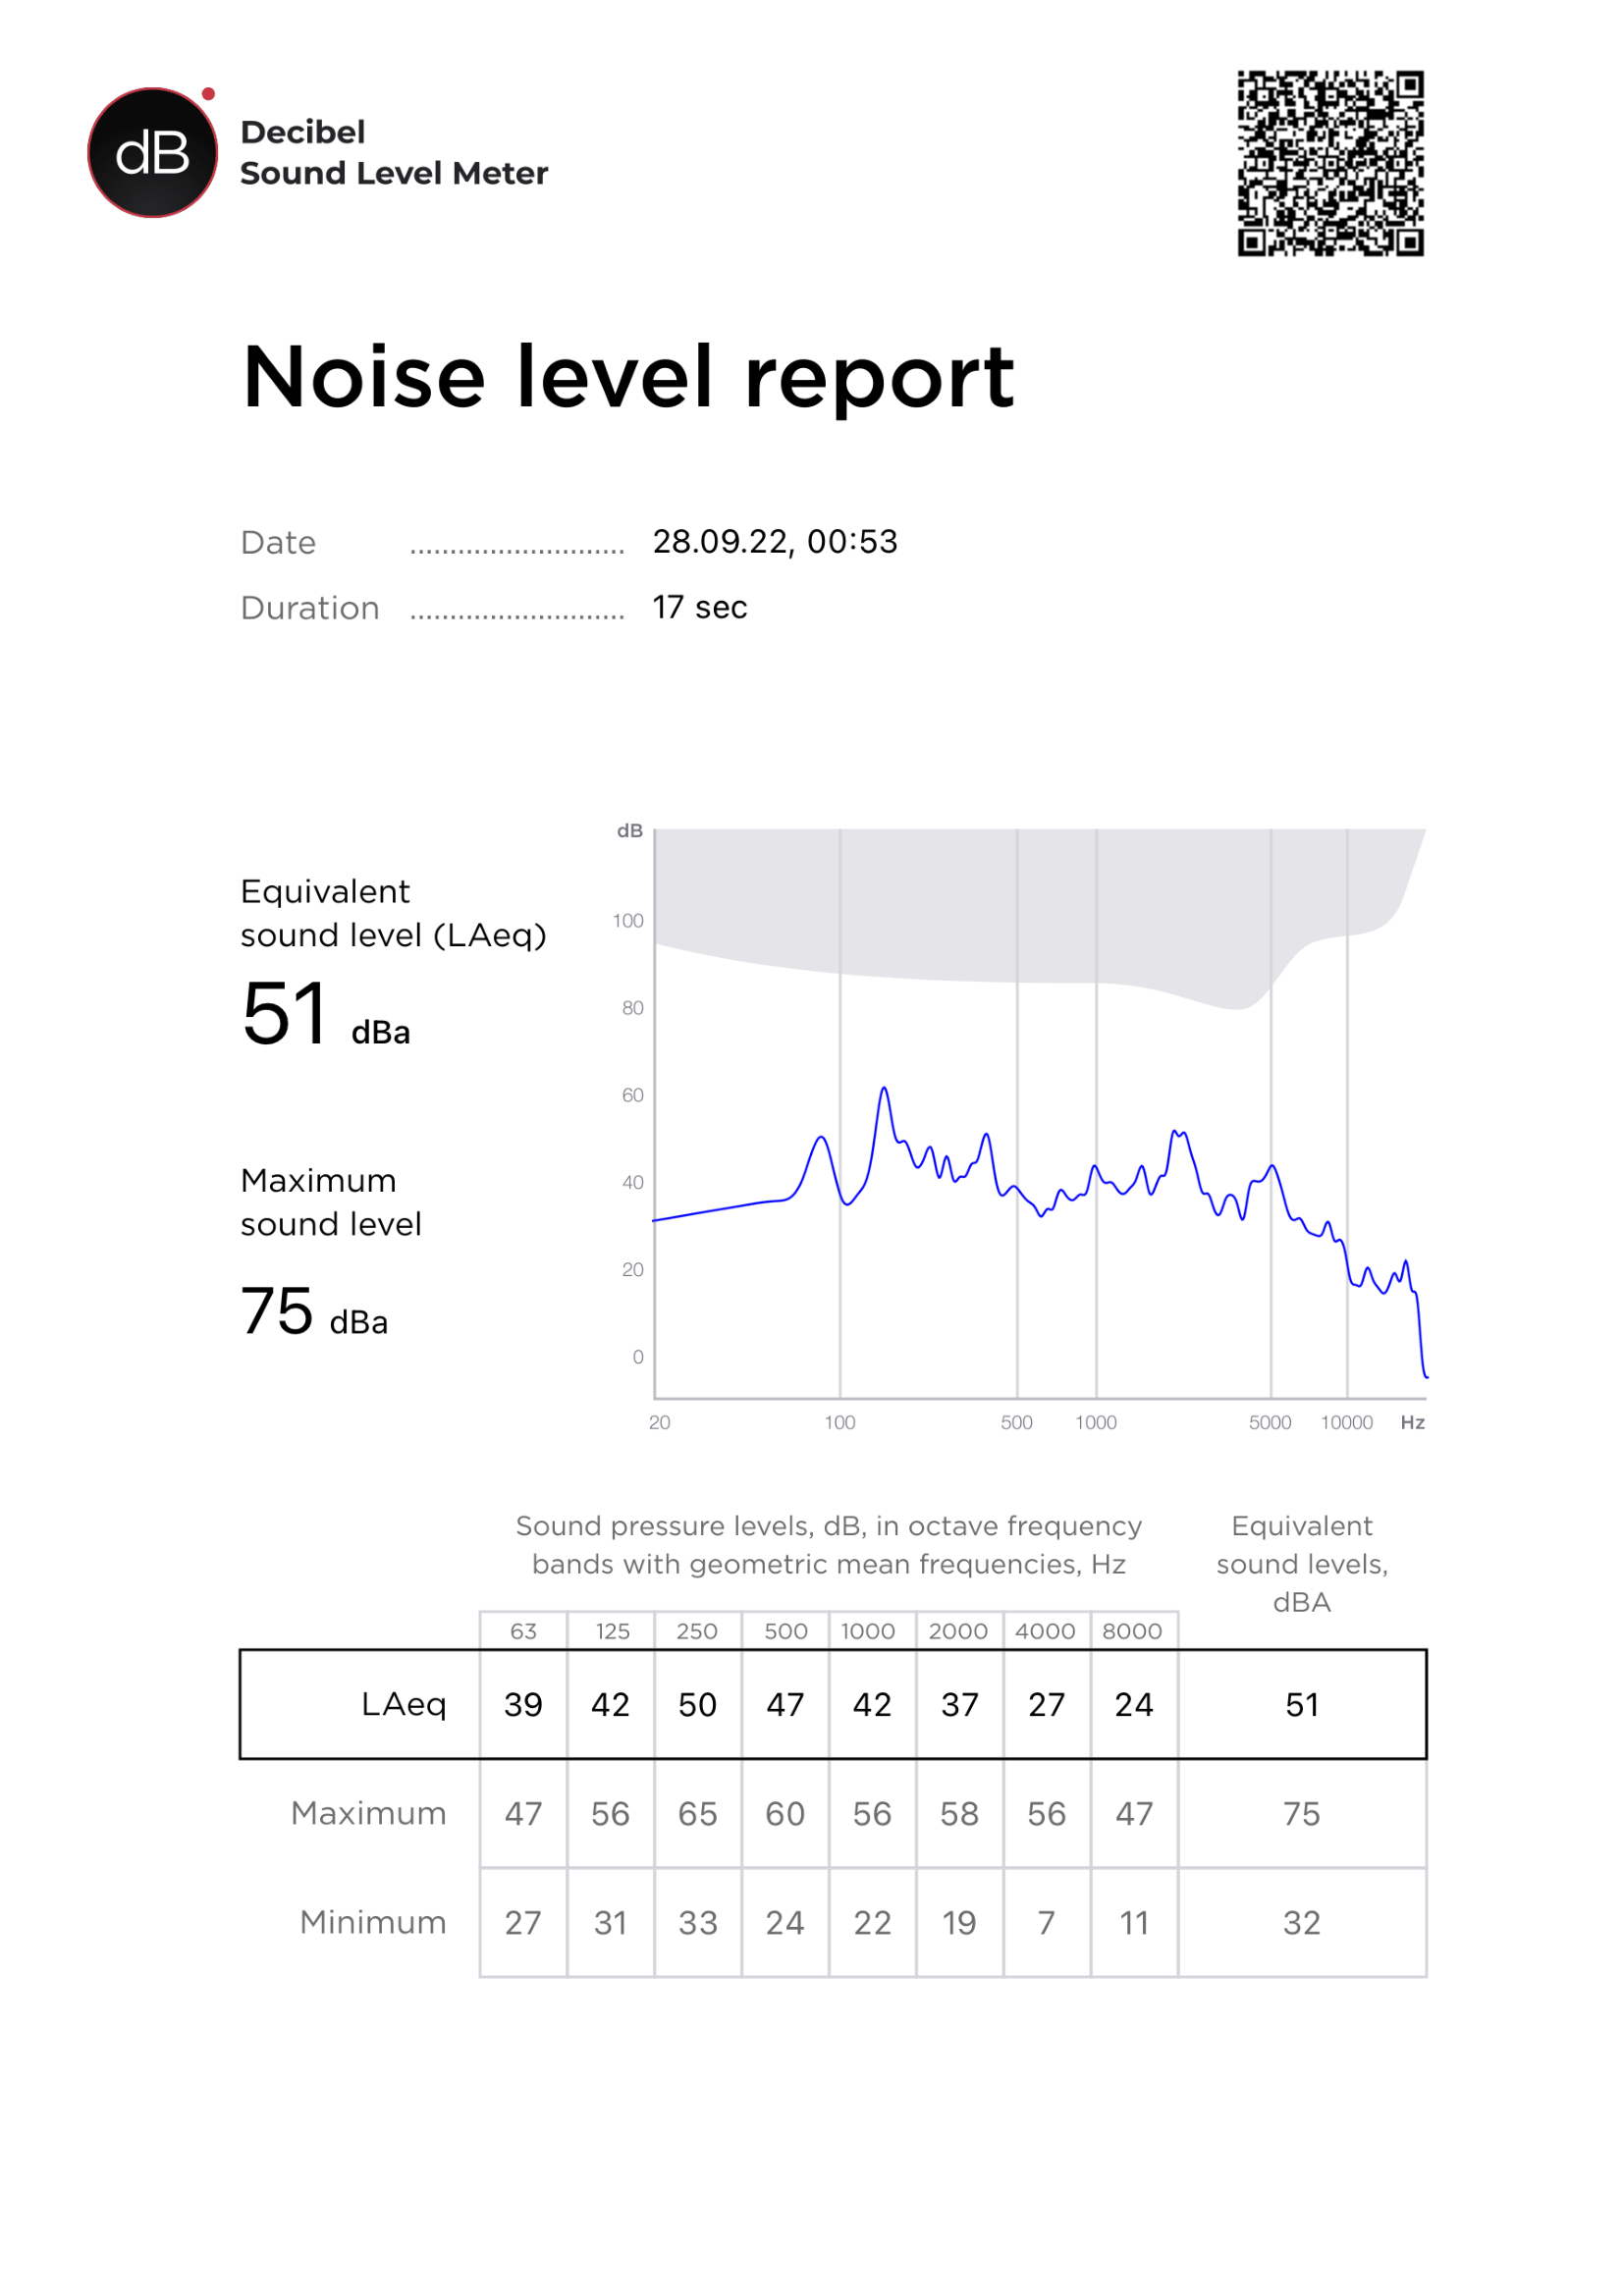
\includegraphics[keepaspectratio, scale=0.6]{data/1.png}
    %\caption{Измерение}
\end{figure}

\begin{figure}[p]
    \centering
    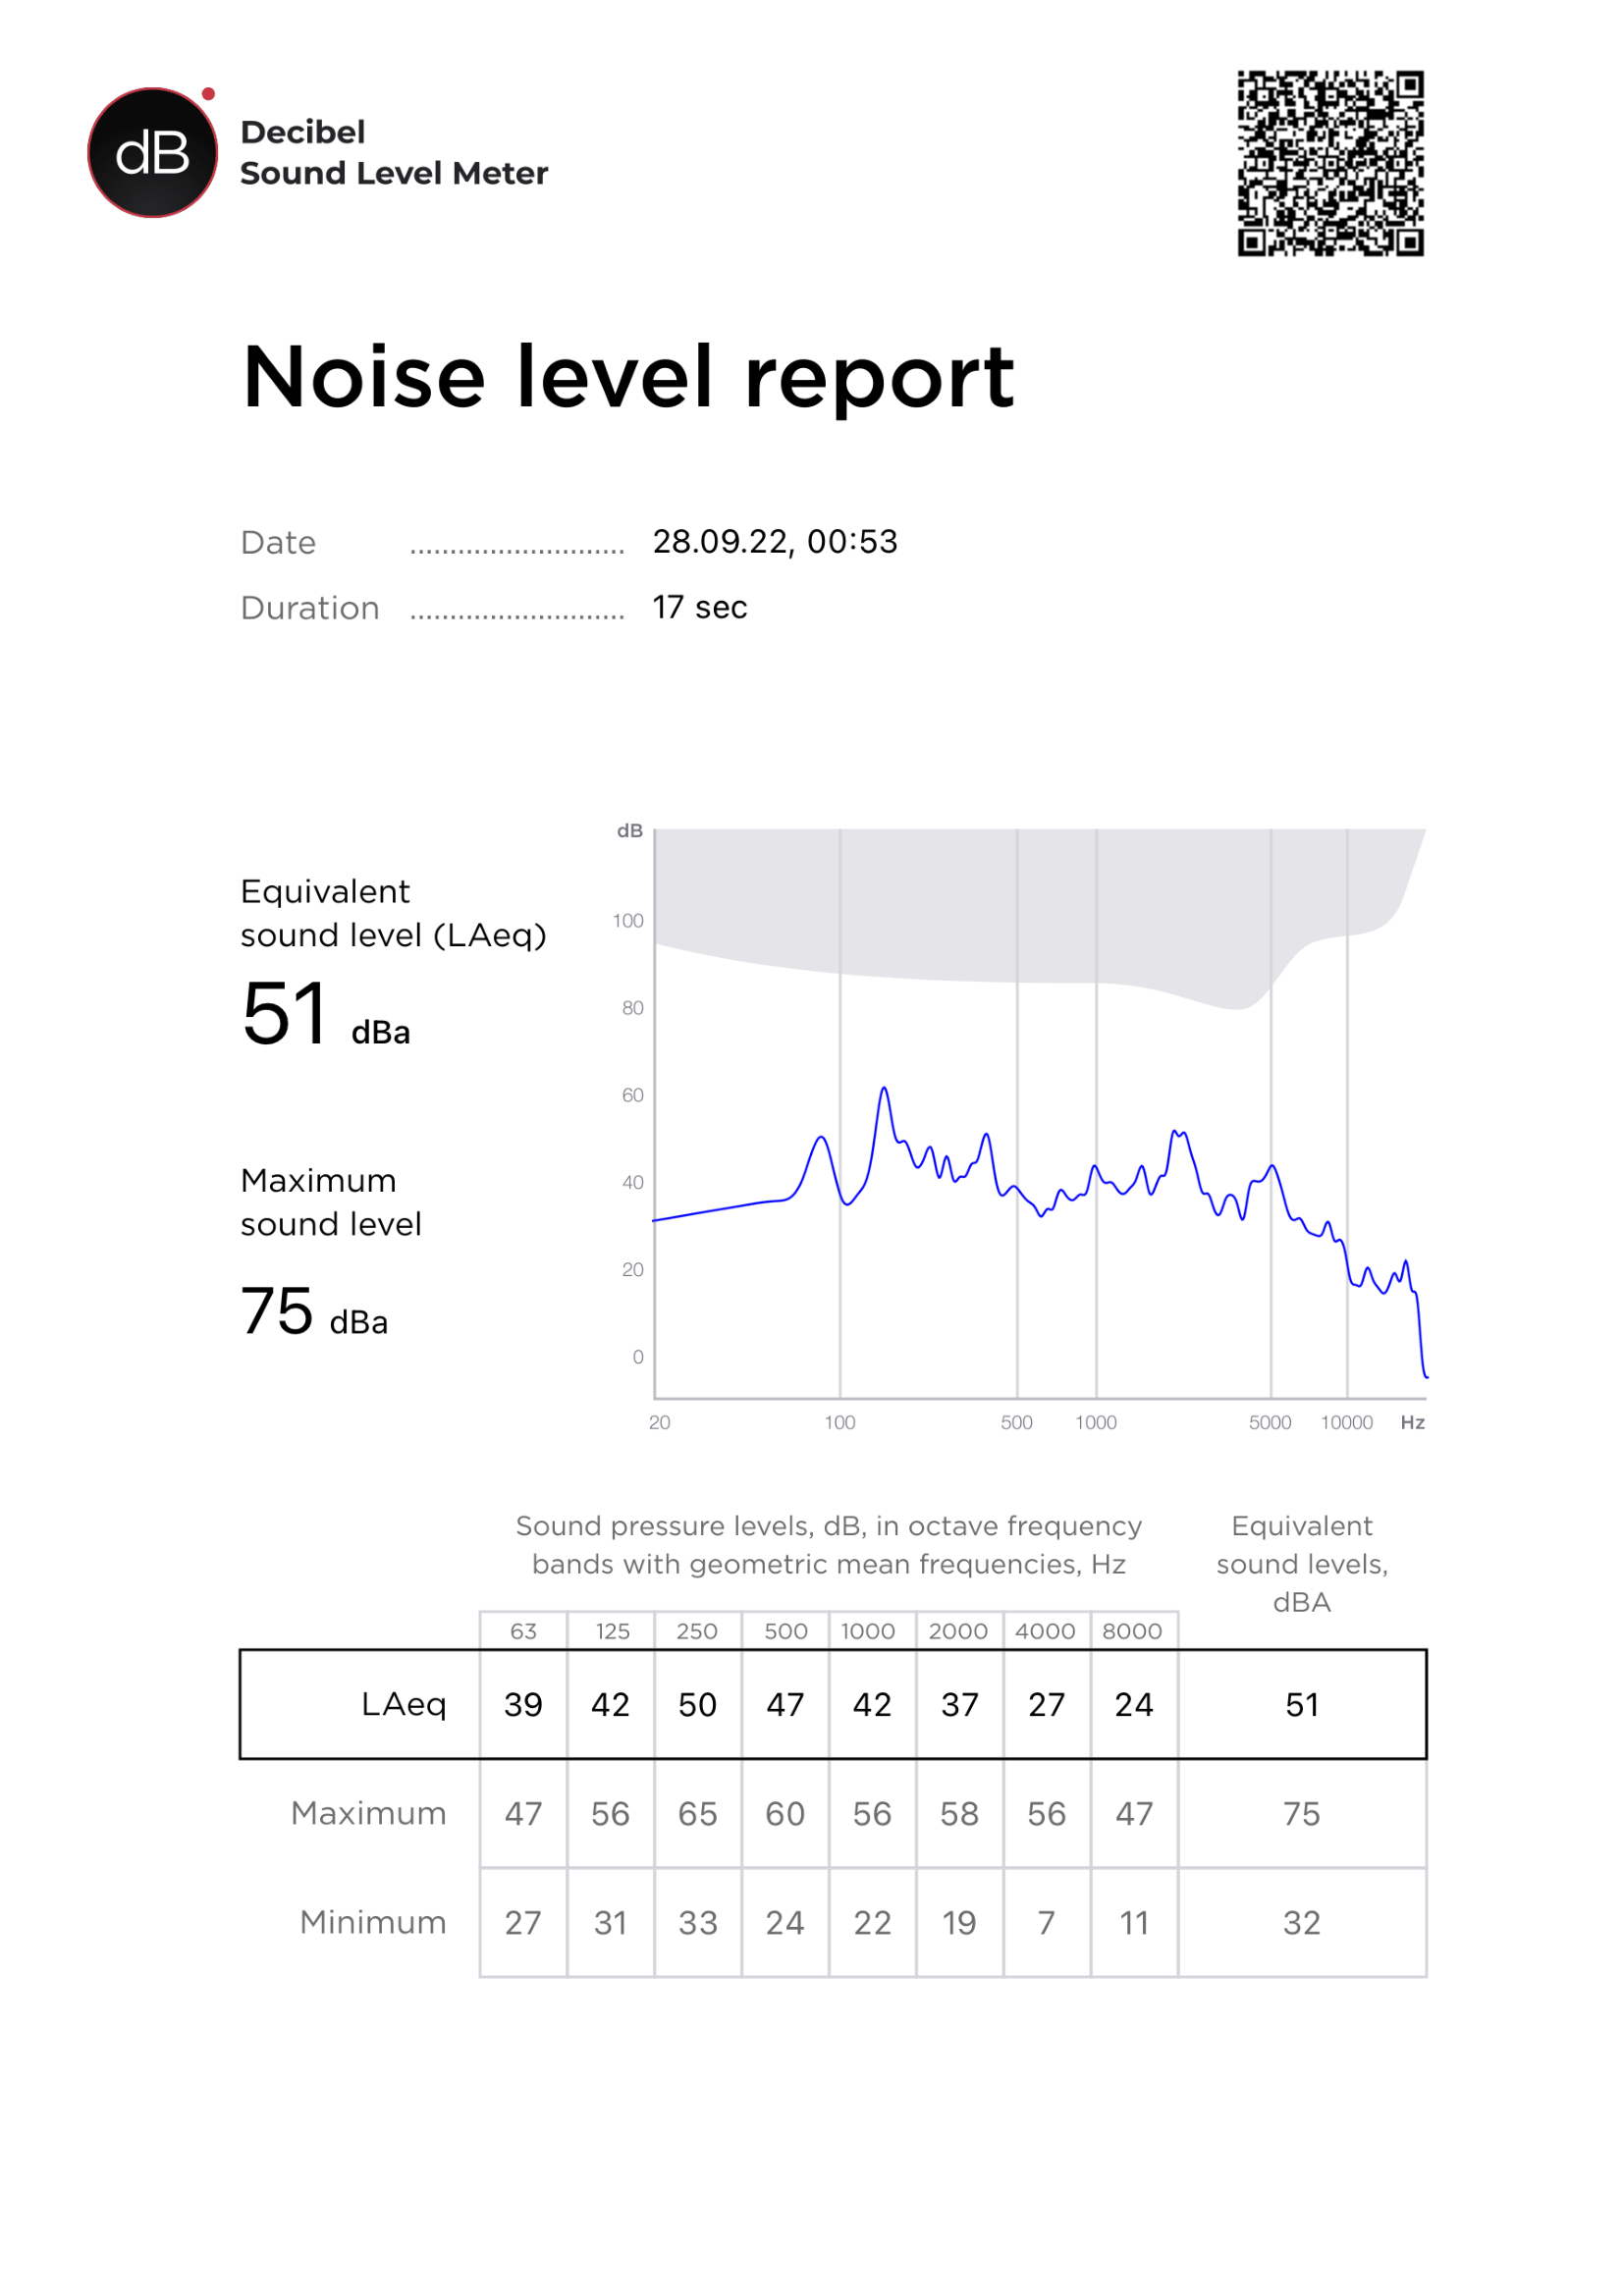
\includegraphics[keepaspectratio, scale=0.6]{data/2.png}
    %\caption{Измерение}
\end{figure}

\begin{figure}[p]
    \centering
    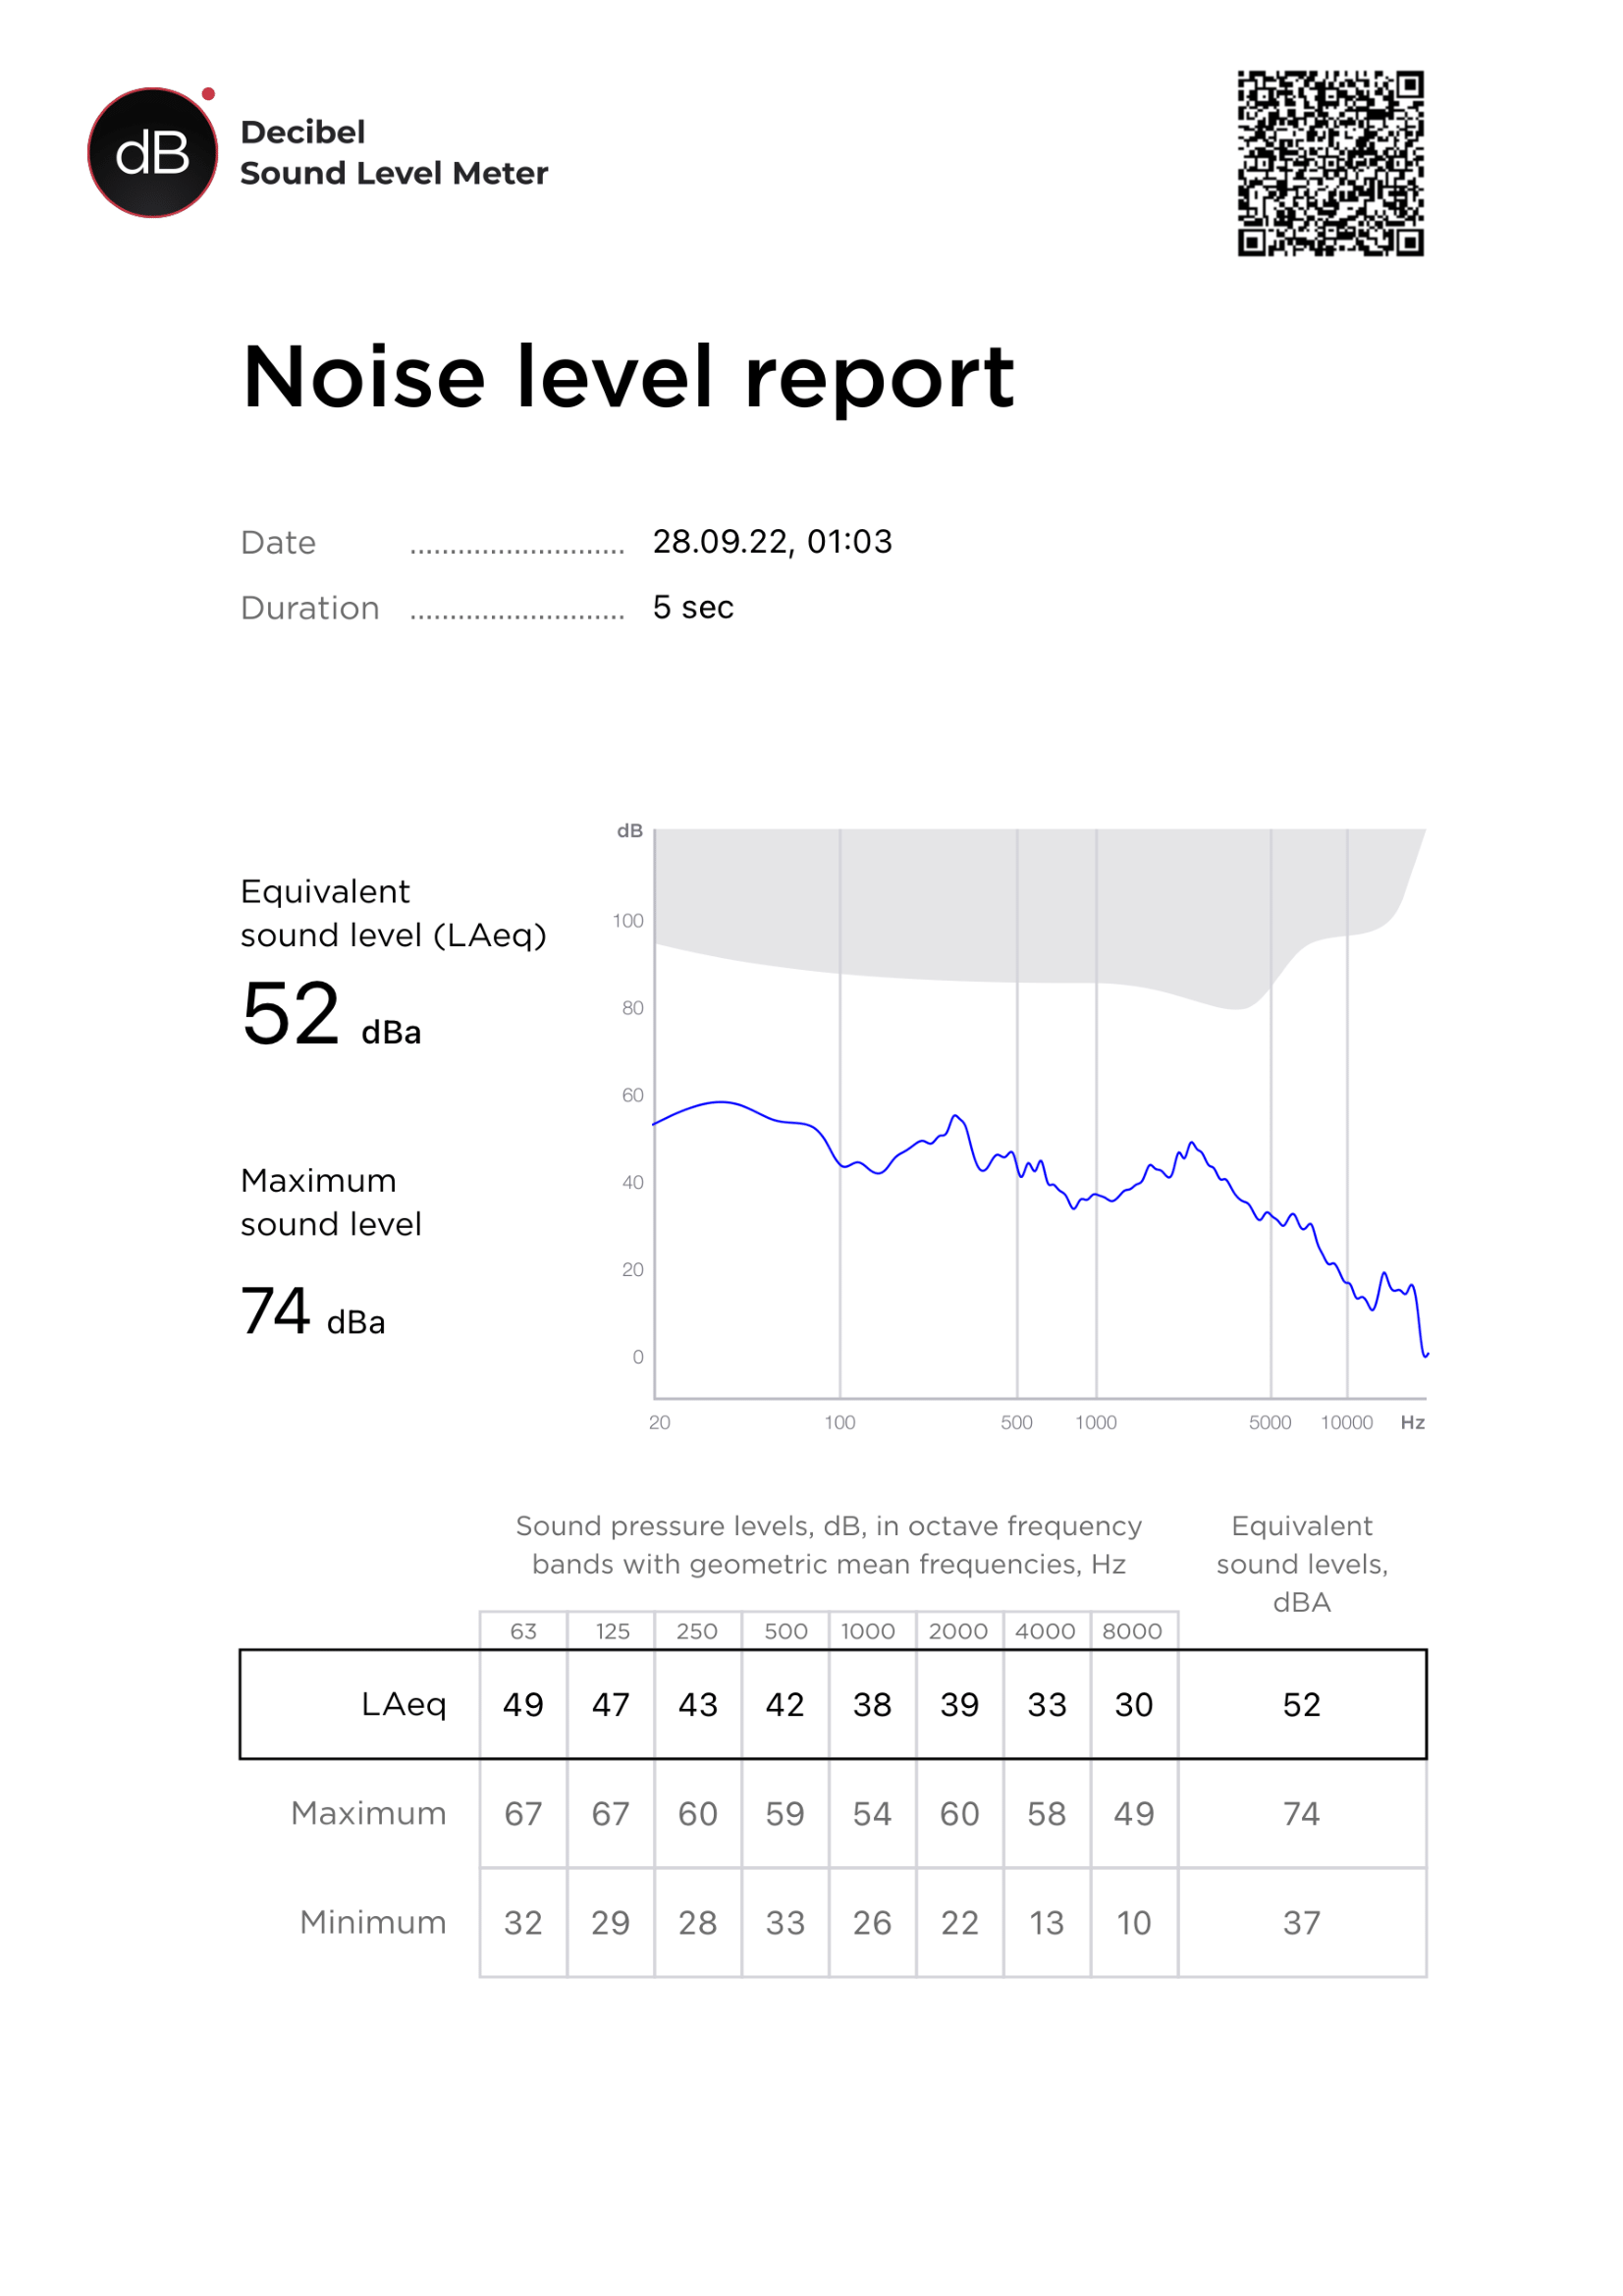
\includegraphics[keepaspectratio, scale=0.6]{data/3.png}
    %\caption{Измерение}
\end{figure}

\subsection*{Вывод}
В ходе выполнения данной практической работы я самостоятельно изучил основные физические характеристики звука, классификацию производственного шума, его вредное действие на организм человека, нормирование, а также получил практические навыки измерений приборами уровней шума от различных источников, произвел расчеты эквивалентного уровня звука на рабочем месте, сравнил эффективность различных методов защиты от производственного шума.
\end{document}